\chapter{Konzept}

\section{Konzept}
Der Pod wird von einem BLDC-Motor angetrieben, wobei die elektrische Energie in einem Lithium-Ionen-Akku gespeichert wird. Der Motor wird durch einen Sinuswellen-Generator gesteuert. Mit dem Speedgoat-System werden die Eingangssignale des Sinuswellen-Generators sowie andere Aktoren gesteuert.

\section{Golden Motor}
\label{Golden_Motor}
Golden Motor ist ein Anbieter von Elektromotoren und elektrischen Antriebssystemen. Das Unternehmen bietet eine breite Palette von Produkten an, darunter:
Motoren und Komplettsysteme für Elektrofahrräder, Industrielle BLDC-Motoren, Elektrische Antriebe für Boote.


\subsection{BLDC Motor}
\label{BLDC_Motor}
Ein BLDC Motor wird mit Gleichspannung angetrieben, wobei eine Leistungssteuerung (Sinuswellen-Generator) die Gleichspannung in ein nutzbares Drehstom umwandelt, dies verhalten wird in Abschnitt \ref{Sinuswellen-Generator} näher erläutert.\\
\begin{figure}[!ht]
	\begin{center}
		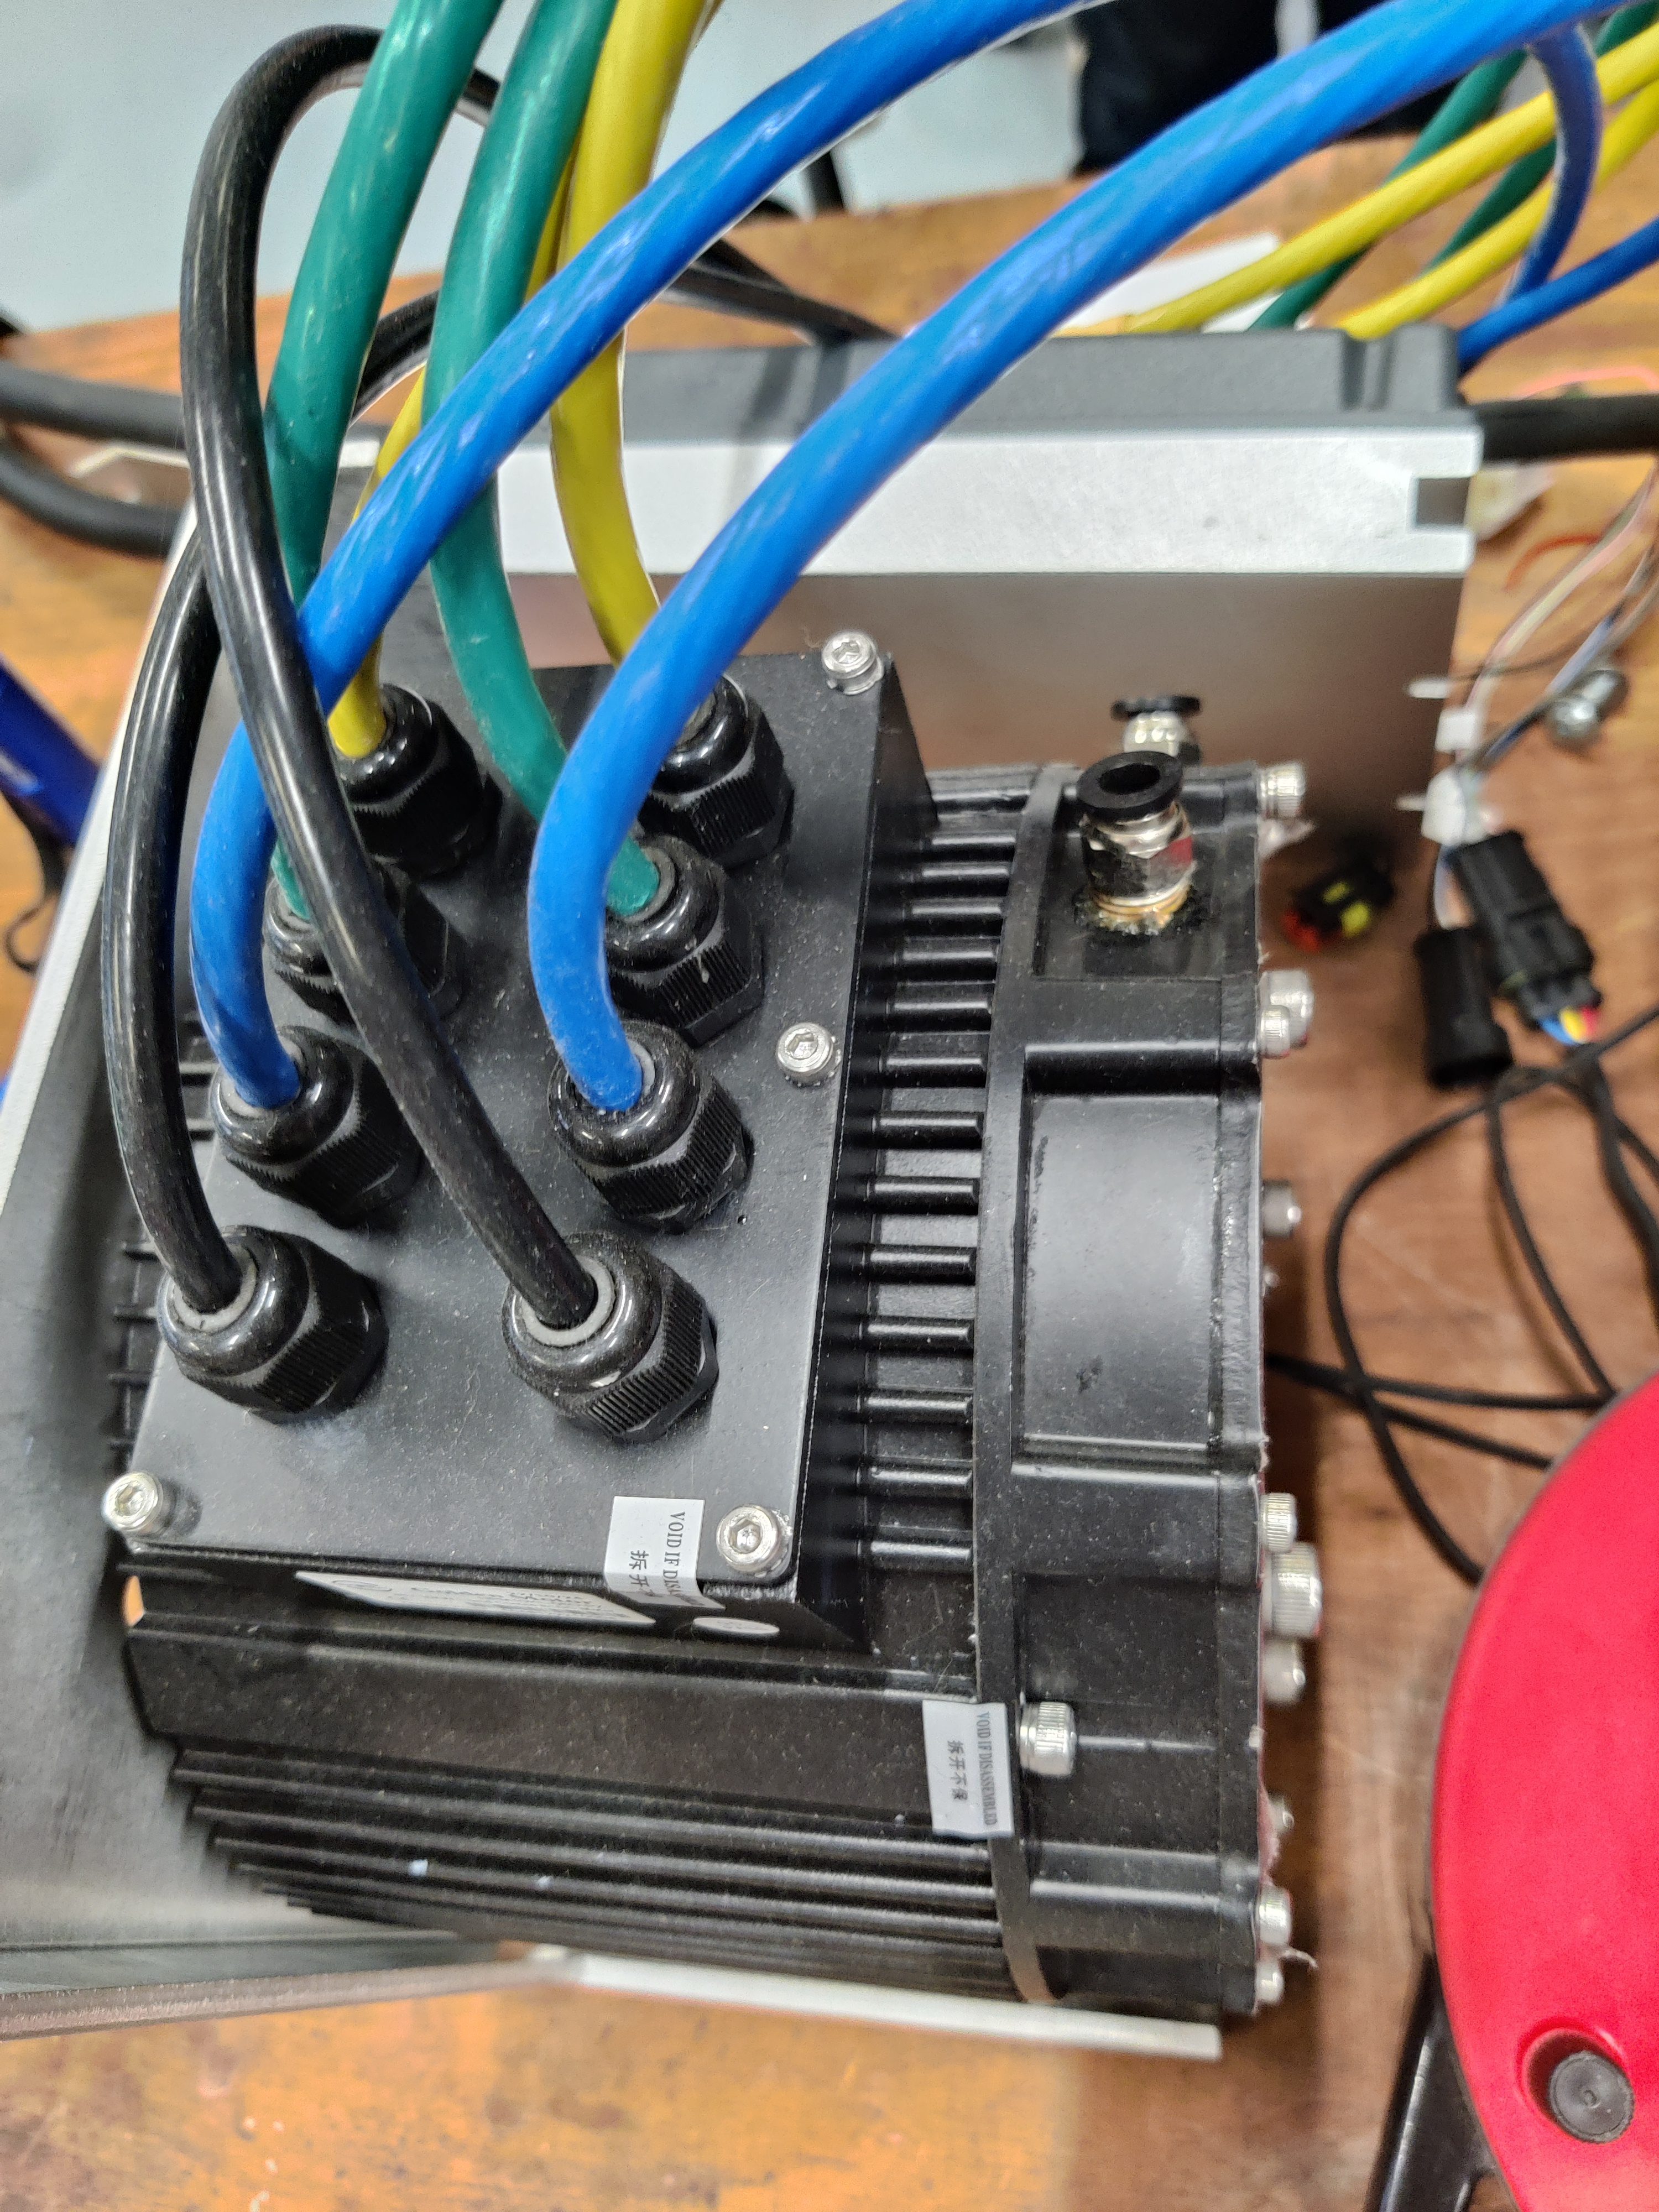
\includegraphics[width=\textwidth]{img/2_imp/2_pic_bldc_motor.png}
		\caption{10 KW BLDC Motor Liquid Cooled}
		\label{img_2_2:motor}
	\end{center}
\end{figure}

Da der Motor keine Schleifkontakte (Kohlebürsten) hat, entsteht kein abrieb. Die Kommutierung, also die Umschaltung der Stromrichtung in den Spulen, erfolgt elektronisch.

Im Rotor (dem rotierenden Teil) befinden sich Permanentmagnete. Im Stator (dem feststehenden Teil) sind Spulen angeordnet. Durch gezieltes Ansteuern der Spulen wird ein magnetisches Drehfeld erzeugt, das den Rotor mit den Permanentmagneten mitnimmt.


\begin{figure}[!ht]
	\begin{center}
		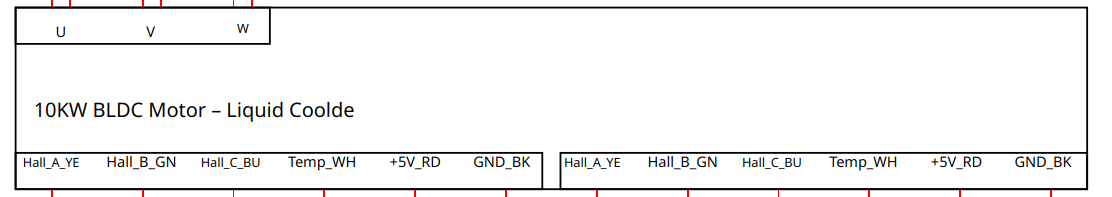
\includegraphics[width=0.75\textwidth]{img/2_imp/2_circ_bldc_motor.png}
		\caption{Zeichnung: BLDC Motor}
		\label{img_2_2:circ_bldc}
	\end{center}
\end{figure}



\subsection{Sinuswellen-Generator}
\label{Sinuswellen-Generator}


%Dafür muss der Abstand ermittelt werden, dies wird mit einem Abstandslaser gemacht.

%Die Steuerung wird als Automaten umgesetzt. Dabei werden unterschiedliche Zustände durchlaufen, wie Idel, Drive, Distance und Stop.


\section{Verdrahtung}

\section{Schaltpaln}

\section{Simulink}

\